\documentclass[12pt,a4paper]{article}

\usepackage[english]{babel}
\usepackage[utf8]{inputenc}
\usepackage{amsmath}
\usepackage{amssymb}
\usepackage{graphicx}
\usepackage{hyperref}
\usepackage{todonotes}
\setuptodonotes{inline}

\begin{document}
\thispagestyle{empty}
\begin{center}
Rheinisch-Westf\"alische Technische Hochschule Aachen \\
Alessandro Berti\\[6ex]

\LARGE
	\textbf{Phase Review: 2nd Sprint of the Implementation of "Conformance Predictions"} \\[6ex]
        \centering{Group 4:}\\
	\textit{Richard Schuppener, Cem Colak} \\[6ex]
\end{center}

\newpage

\tableofcontents
\newpage

\section{Summary of Sprint 2}
In this sprint we focused on the implementation of all the remaining functionalities to have a fully functional end-to-end pipeline for conformance predictions. We intend to use the last sprint to further improve and optimize the functionalities, such that we have a well aligned and polished software artifact at the end of the project, which also fulfills the requirements of Alessandro in the most sophisticated way. 
%%% Mention finalization of documents in sprint 3
 
Key achievements of this sprint include:
\begin{enumerate}
	\item 
\end{enumerate}
\section{Codebase Structure}
We enriched the initial codebase structure, as already outlined in the first sprint review, by a visualization module, which bundles all the visualization functionalities together. 
We decomposed the modules into the following categories: 
\begin{enumerate}
	\item IO: Handle inputs and outputs, such as reading of event logs, normative models, visualization of process models etc.
	\item Feature Extraction: Perform conformance checking (only alignments, thus no separate conformance module), extract features related to alignments, control flow and case attributes and preprocess for ML training (e.g. scaling of numerical values).
	\item Model Training: Properly train a model (as specified by the user) based on the given target and feature vector from the Feature Extraction step. This module also includes the capability to predict unseen data (test data or new data).
	\item Evaluation: Creation of evaluation metrics such as accuracy, precision, recall / fitness, confusion matrix, ROC etc.
	\item Config: Collection of Enums that correspond to the options presented to the user via the CLI. Helps to make the codebase cleaner and better to manage.
	\item Pipeline: In this module, the bigger "steps" of the process bundle functionalities from the previously mentioned modules. Here, based on the choices the user selected, the correct functions are called and inputs, outputs are streamlined together.
	\item Main / CLI: This is the entry point of our program and also serves as the guide and options selector for the user. The CLI presents the user with options, numerical metrics and comprehensive error messages.
	\item Visualization: This module includes all the visualization functionalities. Helps to keep track and adjust the visualizations in a more modular manner.
\end{enumerate}

\section{Requirements Coverage Status - Overview per Module}

\subsection{IO}
\textbf{Covered}
\begin{itemize}
    \item \textbf{LL-01.1}: \texttt{io.discover\_process\_model()} supports Inductive, Alpha, and Genetic Miner via PM4Py, enabling automatic model discovery when no normative model is available.
    \item \textbf{LL-01.2}: \texttt{io.visualize\_process\_model()} renders the model as Petri net, BPMN, or Process Tree, with optional file saving or direct display.
    \item \textbf{HL-05}: Event log loading, model import, and model discovery all functional; the foundational data acquisition step of the pipeline is complete.
    \item \textbf{LL-05.1}: \texttt{pm4py.read\_xes} for XES logs; \texttt{pd.read\_csv} combined with \texttt{pm4py.format\_dataframe} for CSV logs in \texttt{io.load\_event\_log()}.
    \item \textbf{LL-05.2} (partially): Petri net loading via \texttt{pm4py.read\_pnml} implemented; BPMN files loaded via \texttt{pm4py.read\_bpmn} and internally converted to a Petri net.
    \item \textbf{LL-05.3}: Inductive, Alpha, and Genetic Miner available as fallback discovery algorithms when no normative model file is provided.
    \item \textbf{HL-04}: \texttt{try/except} blocks in \texttt{main.py} catch and report setup errors, preprocessing failures, and pipeline exceptions to \texttt{stderr} with descriptive labels.
\end{itemize}

\noindent \textbf{Planned in Sprint 2}
\begin{itemize}
    \item \textbf{HL-01}: End-to-end prediction of conformance deviations as a fully operational business deliverable not yet achieved; requires conformance deviation prediction target to be fully wired through the complete pipeline.
    \item \textbf{LL-05.2}: Standalone loading of BPMN and Process Tree model files as direct model inputs (without forced internal conversion).
\end{itemize}

\subsection{Feature Extraction}

\textbf{Covered}
\begin{itemize}
    \item \textbf{HL-06} (partially): \texttt{feature\_extraction.compute\_alignments()} invokes \texttt{pm4py.conformance\_diagnostics\_alignments}; log-moves, model-moves, and synchronous moves extracted per case. Distance-to-completion indicators not yet included.
    \item \textbf{LL-06.1}: PM4Py alignment dictionaries computed for every trace against the normative Petri net using the standard cost function.
    \item \textbf{LL-06.2}: Alignment moves parsed in \texttt{extract\_label()} to detect and count deviations (log-skips and model-skips) per case; cumulative alignment cost extracted.
    \item \textbf{HL-07} (partially): \texttt{feature\_extraction.extract\_features()} supports control-flow features (Bag-of-Activities), alignment-based diagnostic features (Bag-of-move-types per activity), and a hybrid combination. Case attribute extraction is defined in the code but commented out.
    \item \textbf{LL-07.3}: Control-flow frequency matrix constructed via \texttt{pd.crosstab} over case IDs and activity names, producing a per-case Bag-of-Activities feature matrix.
    \item \textbf{HL-13}: Alignment results computed once per run and stored in-memory; passed as a variable to avoid redundant re-computation within a single pipeline execution.
\end{itemize}


\noindent \textbf{Planned in Sprint 2}
\begin{itemize}
    \item \textbf{HL-02}: Full integration of structured case attributes (e.g., claimant demographics, claim amount) as predictive features alongside process-level signals.
    \item \textbf{HL-06}: Addition of distance-to-completion indicators (e.g., remaining enabled transitions, token distance to final marking).
    \item \textbf{LL-07.1}: Prefix generation loop that slices event sequences to varying lengths $k$ for prefix-level prediction.
    \item \textbf{LL-07.2}: Numerical feature matrix construction tailored to remaining time regression targets.
    \item \textbf{LL-13.1}: Hash-based caching of prefix activity sequences to deterministically identify and skip redundant alignment computations.
    \item \textbf{LL-13.2}: Disk-based persistence of alignment results via \texttt{joblib}.
\end{itemize}

\subsection{Model Training}
\textbf{Covered}
\begin{itemize}
    \item \textbf{HL-08} (partially): \texttt{model\_training.create\_model\_pipeline()} wraps a Decision Tree classifier in a \texttt{sklearn.Pipeline}. Only one algorithm (Decision Tree) currently supported; final alignment cost as deviation threshold not yet used.
    \item \textbf{LL-08.1}: \texttt{StandardScaler} integrated as the first step in the sklearn Pipeline, ensuring scale-consistent feature distributions.
    \item \textbf{HL-09}: Baseline (control-flow features only) and conformance-aware (diagnostics or hybrid features) model variants both supported via the \texttt{PredictionFeature} configuration.
\end{itemize}

\noindent \textbf{Planned in Sprint 2}
\begin{itemize}
    \item \textbf{HL-08}: Use of case final alignment cost as the deviation threshold for defining the binary classification target.
    \item \textbf{LL-08.2}: Additional ML algorithms beyond the Decision Tree (e.g., Random Forest, Logistic Regression) for the controlled comparison.
\end{itemize}

\subsection{Evaluation}

\textbf{Covered}
\begin{itemize}
    \item \textbf{HL-15} (partially): \texttt{evaluation.temporal\_split()} implemented, partitioning cases by end-time into train/val/test sets. The main pipeline currently uses a simplified \texttt{pm4py.split\_train\_test} 75/25 split rather than the full temporal split.
    \item \textbf{HL-16} (partially): \texttt{evaluation.compute\_classification\_metrics()} computes accuracy, precision, recall, F1-score, ROC-AUC, and Brier score for binary and multi-class classification targets.
    \item \textbf{HL-12}: Confusion matrix heatmap and per-class accuracy bar chart generated via Matplotlib in \texttt{evaluation.save\_evaluation\_visuals()}.
\end{itemize}

\noindent \textbf{Planned in Sprint 2}
\begin{itemize}
    \item \textbf{HL-15}: Full integration of \texttt{evaluation.temporal\_split()} into the main pipeline; enforcement of strict temporal case ordering with train, validation, and test sets.
    \item \textbf{HL-16}: Conformance quality metrics for the normative model (fitness, precision, generalization, simplicity).
    \item \textbf{LL-16.2}: MAE and RMSE evaluation metrics for remaining time regression targets.
    \item \textbf{HL-17}: Prefix-length performance analysis using \texttt{evaluation.evaluate\_by\_prefix\_length()} (function stub already present).
\end{itemize}

\subsection{Config \& Pipeline}

\textbf{Covered}
\begin{itemize}
    \item \textbf{HL-03} (partially): \texttt{main.py} provides an interactive CLI guiding the user through model path/discovery selection, prediction target (future deviations, process outcome, remaining time), feature basis, and ML algorithm configuration. Conformance deviations as target and case attributes as feature basis not fully functional end-to-end.
    \item \textbf{LL-03.1} (partially): Prediction target and feature basis options fully defined in \texttt{config.py} and selectable in the CLI; case attribute extraction and conformance deviation target not yet fully wired through the pipeline.
    \item \textbf{HL-10}: \texttt{main.py} combined with \texttt{pipeline.py} forms an end-to-end runner from raw data and model input to evaluation output, without manual intermediate steps.
\end{itemize}

\noindent \textbf{Planned in Sprint 2}
\begin{itemize}
    \item \textbf{HL-03}: Full CLI support for conformance deviations as prediction target and case attributes as feature basis.
    \item \textbf{HL-14}: Runtime and resource measurement wrapping conformance checking and feature generation steps.
    \item \textbf{LL-14.1}: \texttt{time.perf\_counter()} timing instrumented around alignment computation and model training calls.
    \item \textbf{LL-14.2}: \texttt{psutil.Process().memory\_info()} peak RAM tracking during preprocessing and alignment.
    \item \textbf{LL-14.3}: Millisecond-level start/end timestamps recorded per batch for the combined conformance checking and feature generation steps.
    \item \textbf{LL-14.4}: Runtime and resource metrics printed to the console and persisted in a structured log file (CSV or JSON).
\end{itemize}

\subsection{Project Infrastructure \& Testing}
\textbf{Covered}
\begin{itemize}
    \item \textbf{HL-18}: PM4Py, scikit-learn, pandas, NumPy, and Matplotlib used as the primary library stack throughout all modules.
    \item \textbf{HL-19 \& LL-19.1-19.2}: Project organized into \texttt{io}, \texttt{feature\_extraction}, \texttt{model\_training}, \texttt{evaluation}, \texttt{pipeline}, and centralized \texttt{config} modules; Git used for version control. Note: conformance logic currently consolidated into \texttt{feature\_extraction} rather than a dedicated \texttt{conformance} module. Branching strategy for each module not considered, as we are working on two branches for each team member.
    \item \textbf{HL-20}: \texttt{requirements.txt} and \texttt{README.md} present in the repository.
    \item \textbf{HL-20.1}: \texttt{requirements.txt} as a plain text file implemented and considered satisfactory for dependency management so far.
\end{itemize}

\noindent \textbf{Planned in Sprint 2}
\begin{itemize}
    \item \textbf{HL-11}: Automated pytest test suite executable via a single command.
    \item \textbf{LL-11.1}: Pytest fixtures providing a synthetic, fully conforming XES log and corresponding Petri net.
    \item \textbf{LL-11.2}: Test assertion that alignment cost equals $0.0$ on fully conforming synthetic data.
    \item \textbf{LL-11.3}: Test assertion that a prefix of length $k$ contains strictly only the first $k$ events of the original trace.
    \item \textbf{HL-21}: Technical documentation of system architecture, data and model flow, conformance checking strategy, feature design, and main implementation choices. An architecture diagram is considered as a key component of this documentation.
\end{itemize}

\section{User Guide}
% Not updated, meistens gleich geblieben und eigentlich selbsterklärend 
% Planned to write a comprehensive user guide 
\section{Team settings and Workflow}
\subsection{Changes in Responsibilities}
As already stated in the first sprint review, we changed the responsibilities in this sprint. In this sprint, Cem was responsible for I/O, Model Training and Feature Extraction. Richard was responsible for the new visualization module, evaluation and pipeline. Both of us were responsible for the CLI and config module, as they are relatively small and we wanted to work on them together to have a common understanding of the user interface and configuration options. We think this division of responsibilities worked well, as it allowed us to understand and reflect on each others past contributions and contribute with new capabilities.

For the incoming sprint, we plan to keep the split and set a stronger focus on the documentation. We intend to work together on the User Guide, technical documentation, Read Me, and the phase review.
% Mention that we keep the split and eventually work cross, especially in terms of the documents

\subsection{Workflow Improvements for the next sprint}
In this sprint, we changed our branching and workflow strategy. First, we implemented a more granular decomposition of the work items in git, such that we were able to precisely adopt the planned requirements for this sprint. Second, we consolidated the personal branches into the key branches "development", "documents" and "main", and created branches for the work items we were working on. Later we merged these work item-based branches into their respective parents. 
%%more documentation and issue based workflow in git

\section{Exemplary Visualizations and Outputs}
In this section a select sample of visualizations is included. The pipeline was run with the \textit{sepsis-cases} event log and following parameters:
\begin{itemize}
	\item Discovery Algorithm: Inductive Miner (noise threshold = 0.1)
	\item Target: Process outcome
	\item Outcome activities: Release A-E
	\item ML-Algorithm: Decision Tree
\end{itemize}
The confusion matrix was derived from a run with $prefix length = 8$, \textit{control flow} as feature and decision tree depth of 4. 
The decision tree stems from a run with $prefix length = 5$, \textit{control flow}, and the decision tree depth being capped to 3.
The graph depicting average class accuracy was derived from a run with $prefix length = 8$ and \textit{Diagnostics} (= Control Flow + Alignments) as feature and decision tree depth of 4.
Interestingly, including information about alignments helped the decision tree correctly classify other outcomes than the majority label, but did not necessarily greatly improve overall accuracy. In general, having longer prefixes greatly improved the evaluation metrics. We believe this has to do with the following:
\begin{enumerate}
	\item Process outcome is more likely to be actually contained in the trace prefix (data leakage $\rightarrow$ currently no countermeasure implemented)
	\item Smaller prefixes reduce the number of variants greatly $\rightarrow$ smaller training set.
\end{enumerate}
We also integrated the PM4Py visualization of \textit{Process Trees} and \textit{BPMN}.
\begin{figure}[htbp]
	\centering
	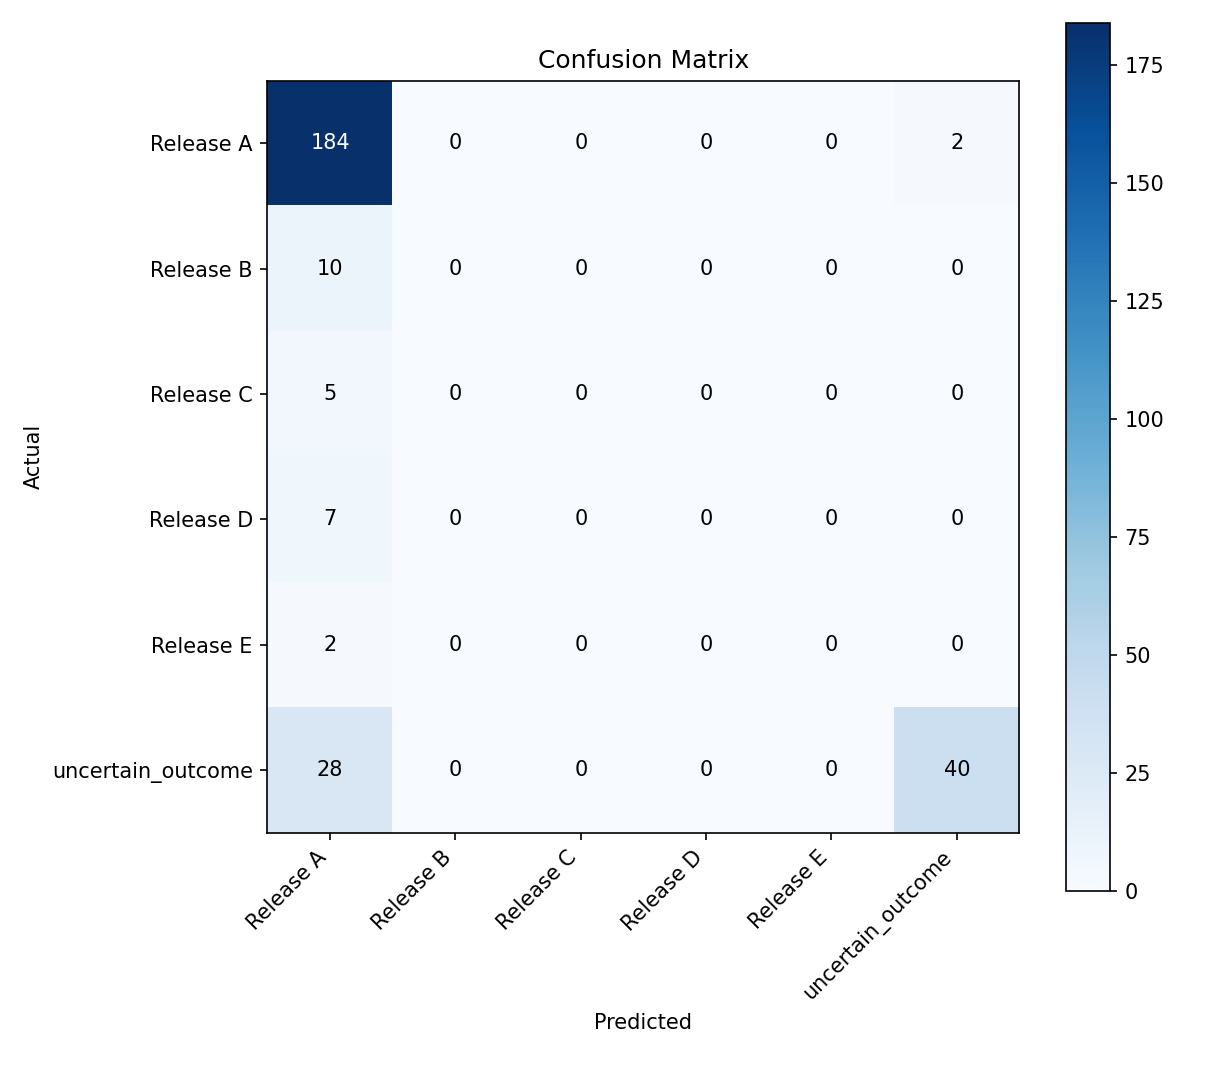
\includegraphics[width=\textwidth]{figures/confusion_matrix.png}
	\caption{Confusion matrix visualization.}
\end{figure}
\begin{figure}[htbp]
	\centering
	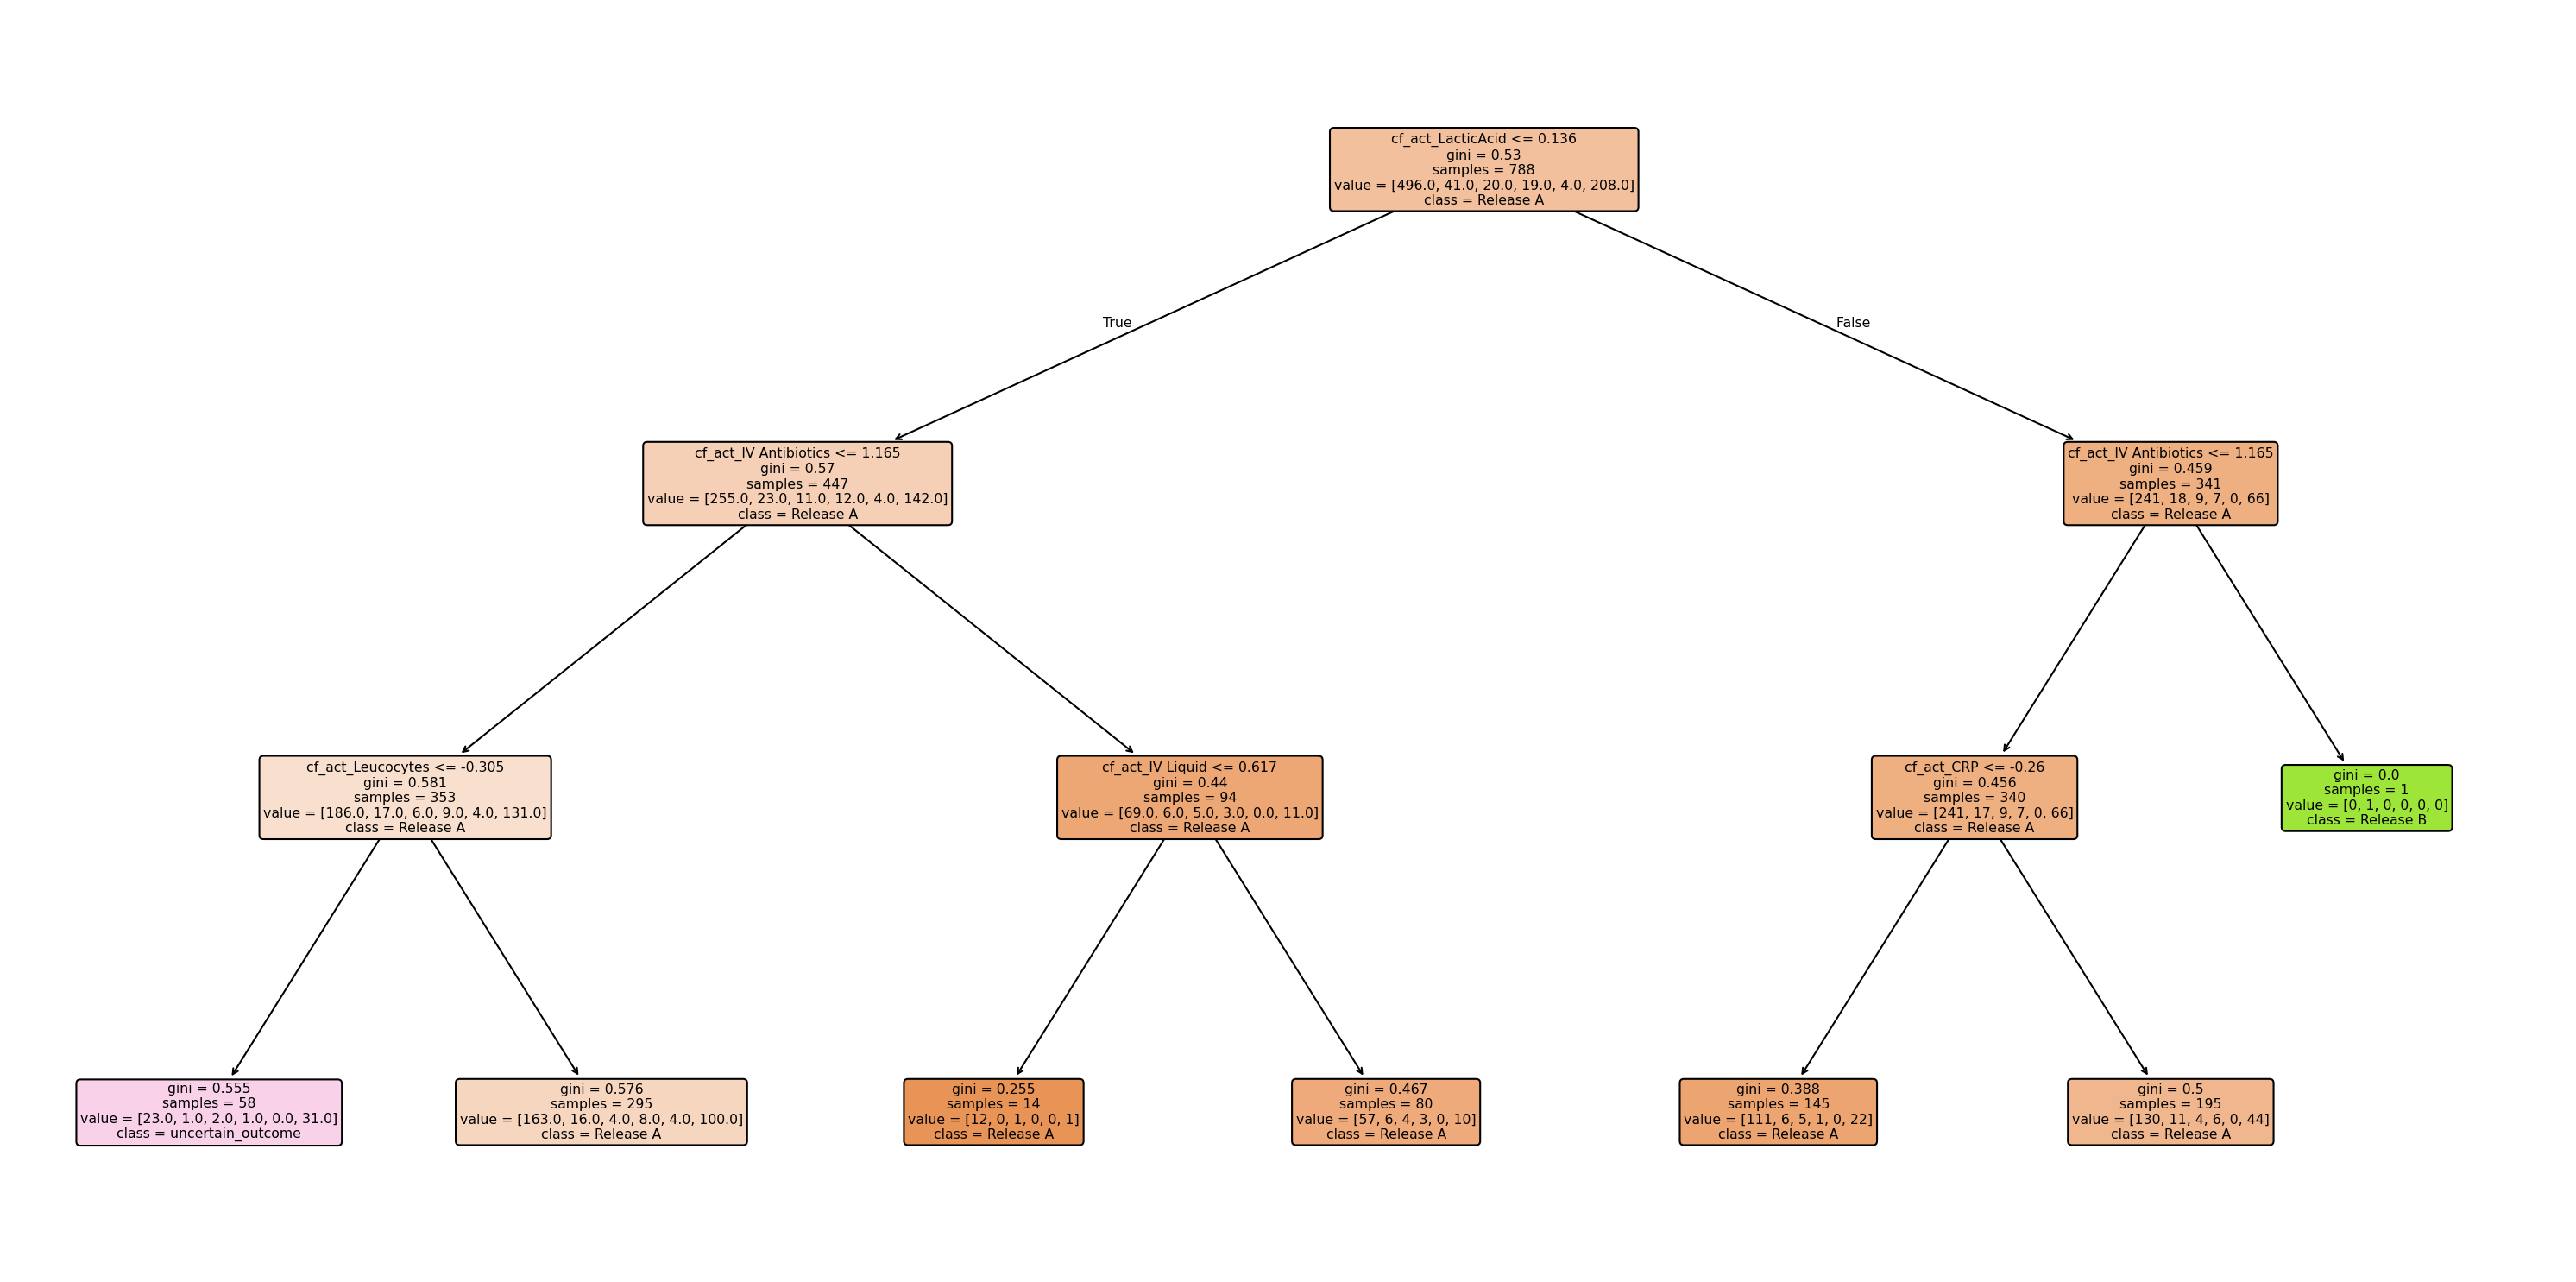
\includegraphics[width=\textwidth]{figures/decision_tree.png}
	\caption{Decision tree visualization.}
\end{figure}
\begin{figure}[htbp]
	\centering
	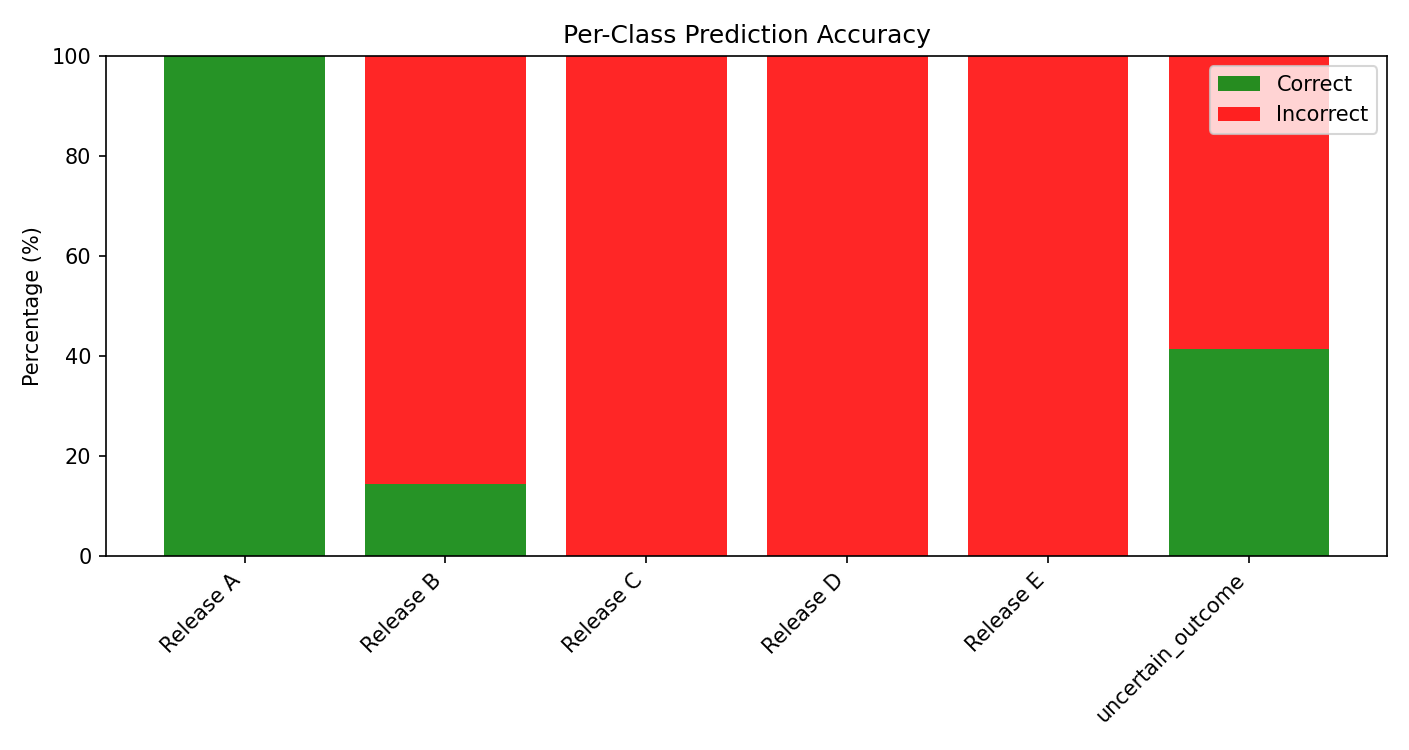
\includegraphics[width=\textwidth]{figures/per_class_accuracy.png}
	\caption{Accuracy per class graph.}
\end{figure}
\begin{figure}[htbp]
	\centering
	\includegraphics[width=\textwidth]{figures/process_model.png}
	\caption{PM4Py petri net visualization.}
\end{figure}

\section{Sprint review}

\subsection{Richard Schuppener}
\todo{review}
\subsection{Cem Colak}
\todo{review}
\end{document}
